\chapter{Introdution to Java}
\label{ch:java}
\markboth{Introdution to Java}{}


\begin{flushright}
	{\smaller
		\textit{Language is only the instrument of science, \\and words are but the signs of ideas.}\\
		-- Samuel Johnson}
\end{flushright}


\section{The java Language}
The term Java refers both to a programming language with the higher number of developers in the worldwide and to a technology that has several sub-technologies that have emerged in different fields of use of the software. Javawas developed by Sun Microsystems, a company that was incorporated in Oracle from a few years.
In 1996, James Gosling, Bill Joy, and Guy Steele wrote for the First Edition of The Java Language Specification:
``{\itshape We believe that the Java programming language is a mature language, ready for widespread use. Nevertheless, we expect some evolution of the language in the years to come. We intend to manage this evolution in a way that is completely compatible with existing applications.}''\\
This programming language is a general-purpose, concurrent, classbased, object-oriented language. It is designed to be simple enough that many programmers can achieve fluency in the language.\cite{javaoracle}
One design goal of Java is portability, which means that programs written for the Java platform must run similarly on any combination of hardware and operating system with adequate runtime support. This is achieved by compiling the Java language code to an intermediate representation called Java bytecode, instead of directly to architecture-specific machine code. Java bytecode instructions are analogous to machine code, but they are intended to be executed by a virtual machine (VM) written specifically for the host hardware. End users commonly use a Java Runtime Environment (JRE) installed on their own machine for standalone Java applications, or in a web browser for Java applets.\cite{wiki:java}
Standard libraries provide a generic way to access host-specific features such as graphics, threading, and networking.\\
There were five primary goals in the creation of the Java language:\cite{java}
\begin{enumerate}
\item It must be ``simple, object-oriented, and familiar''.
\item It must be ``robust and secure''.
\item It must be ``architecture-neutral and portable''.
\item It must execute with ``high performance''.
\item It must be ``interpreted, threaded, and dynamic''.
\end{enumerate}
Java SE 8 represents the single largest evolution of the Java language in its history. A relatively small number of features - lambda expressions, method references, and functional interfaces - combine to offer a programming model that fuses the objectoriented
and functional styles. Under the leadership of Brian Goetz, this fusion has been accomplished in a way that encourages best practices - immutability, statelessness, compositionality - while preserving ``the feel of Java'' - readability, simplicity, universality.\\
Actually Java is the most used programming language according to TIOBE. The TIOBE Programming Community index is an indicator of the popularity of programming languages. The ratings are based on the number of skilled engineers world-wide, courses and third party vendors.


\section{Java choice}

The software presented in this thesis work is completely written in Java. The choice of the programming language was driven by several considerations. These include the following:

\begin{itemize}
\item the language should be widely supported; this to avoid the case of many valid aircraft design applications and libraries that became obsolete due to the aging of the programming language used to build them;
\item the language should promote the use of open source libraries, especially for I/O tasks and for complex mathematical operations;
\item the language and the companion \gls{acr:ide} should provide a widely supported \gls{GUI} framework and a \gls{GUI} visual builder;
\item  the language should support and promote modularity.
\end{itemize}
The Java programming language meets all these requirements: it is backed by Oracle and by a huge community of developers so it is continuously updated. Also, advanced and free \gls{acr:ide}s (such as Eclipse) allow programmers to streamline and simplify the development process. In particular, the Eclipse \gls{acr:ide} and the SWT/JFace libraries have been chosen to develop \gls{acr:Jpad} and its \gls{GUI}.
Being Java a pure object oriented programming language, it greatly encourages and simplifies modularization. Each module (package) can be programmed quite independently so that it is relatively easy to divide the work among several programmers. This is essential since the amount of classes and calculations needed to abstract, manage and analyze the entire aircraft is very large (presently the whole project counts more than 56000 lines of code). For such a reason the establishment of common practices and the adherence to fundamental principle of software development (Don’t Repeat Yourself, Separation of Concerns, Agile software development) are equally important.
An important design requirement of \gls{acr:Adopt} is related to its interoperability with other engineering analysis tools. In fact, the application can be easily integrated into a comprehensive aircraft optimization cycle. This is made possible because \gls{acr:Adopt} can be launched both in \gls{GUI} and command line mode. Much care has been given to input/output and configuration files to increase the possible uses of the software.\cite{adoptunina}

\begin{figure}[H]
\centering
{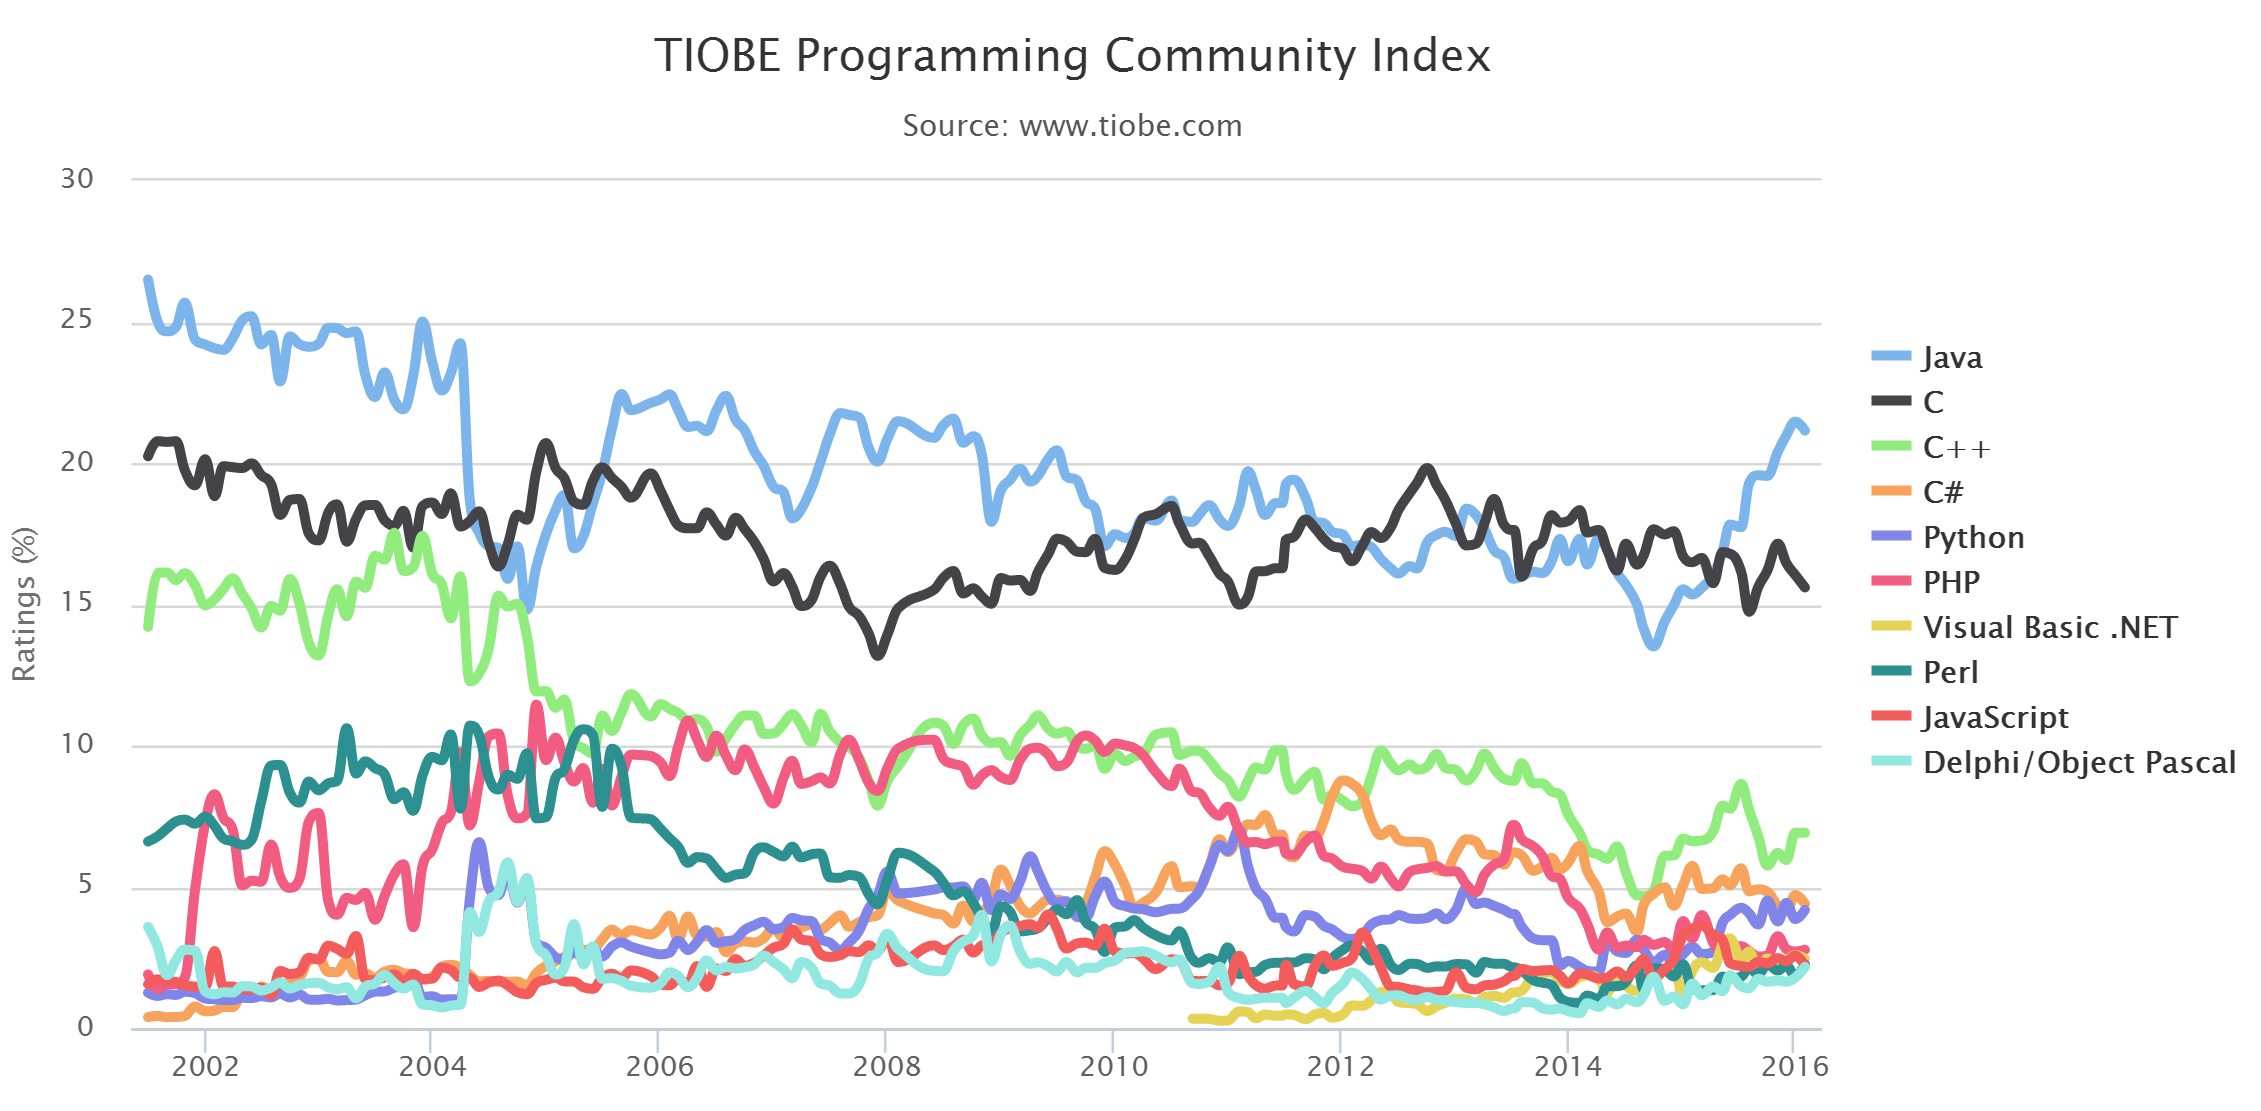
\includegraphics[height=7.6cm ]{Immagini/trend.png}} 
\caption{Programming Language popularity trade.}
\label{fig:hl}
\end{figure}






